%------------------------------------------------
%
% Structure.tex
%
% This file contains the structure of the
% designed Service Desk
%------------------------------------------------
\section[Struttura del Service Desk]{struttura del service desk}
\label{sd-structure}
L'\entity{} è strutturato su due presidi (visibili in Figura \ref{sd-structure-maps}) con destinazione d'uso specifica:

\begin{enumerate}
\item{la sede principale (Piazza Cardinal Ferrari):}
\begin{itemize}
\item{padiglione ``principe di Piemonte'';}
\item{monoblocco A;}
\item{monoblocco B;}
\item{palazzina uffici;}
\item{ex convitto infermieri.}
\end{itemize}
\item{sede secondaria di via Isocrate:}
\begin{itemize}
\item{rifugio Fanny Finzi Ottolenghi}
\end{itemize}
\end{enumerate}

A seguito di una supervisione dei locali e dopo aver valutato come sono suddivise le risorse (vedi Sezione \ref{sd-resources}) sui diversi presidi si ritiene adeguata l'implementazione di un \keyword{\english{Service Desk} centralizzato}.

La posizione fisica che presenta le caratteristiche più idonee è situata nel primo presidio all'interno della palazzina in cui risiedono gli uffici.

Le motivazioni che hanno condotto il proponente verso questa scelta sono le seguenti:

\begin{itemize}
\item{dimensione della struttura;}
\item{gestione delle risorse;}
\item{posizione geografica dei presidi.}
\end{itemize}

\begin{figure}[htbp]
\centering
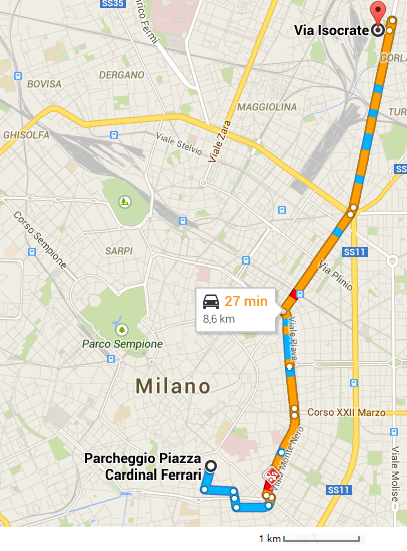
\includegraphics[scale=0.6]{Images/maps.png}
\caption{Posizione geografica dei presidi}
\label{sd-structure-maps}
\end{figure}

\subsection[Dimensione della struttura]{dimensione della struttura}
\label{sd-structure-size}
Considerando che l'intera struttura ospedaliera è collocata all'interno del medesimo comune (seppur di grandi dimensioni), la duplicazione della funzione di \english{Service Desk} su entrambi i presidi è da sconsigliarsi in quanto essi sono a pochi Km di distanza l'uno dall'altro.

Considerando inoltre che la maggior parte delle risorse (\english{software} ed \english{hardware}) sono collocate all'interno della sede principale e, la duplicazione non porterebbe alcun beneficio ma solo una duplicazione dei costi di gestione.

\subsection[Gestione delle risorse]{gestione delle risorse}
\label{sd-structure-resource-management}
Attraverso una singola sede centralizzata è possibile gestire in modo \keyword{più efficiente} e \keyword{più economico} le risorse di cui l'istituto dispone.

Consente inoltre un \keyword{risparmio} nell'acquisto di nuove risorse (\english{software} ed \english{hardware}) poiché queste non dovranno essere replicate come nel caso di sedi separate del \english{Service Desk}.

\subsection[Posizione geografica]{posizione geografica}
\label{sd-structure-position}
Considerando che i presidi dell'\entity{} distano pochi Km l'uno dall'altro (poco meno di 10Km) la collocazione di un unica sede del \english{Service Desk} all'interno del primo presidio farà comunque beneficiare, alla struttura ospedaliera, dei benefici offerti da un \english{Service Desk} di tipo locale.

Quali:

\begin{itemize}
\item{fornitura di una presenza visibile agli utenti;}
\item{comunicazione con lo staff semplificata.}
\end{itemize}